\subsection{Aplicação Fábrica: Executar Analise}
\subsubsection*{Descrição do caso de uso}
Uma analise é um \textit{script} SQL com uma \textit{query} personalizada. Para executar uma analise basta pressionar o botão \textit{executar} na linha referente à analise pretendida. A aparência da \textit{view} deste caso de utilização será semelhante ao demonstrado na figura \ref{fig:di_analise}.

\begin{figure}[H] 
	\begin{center}
		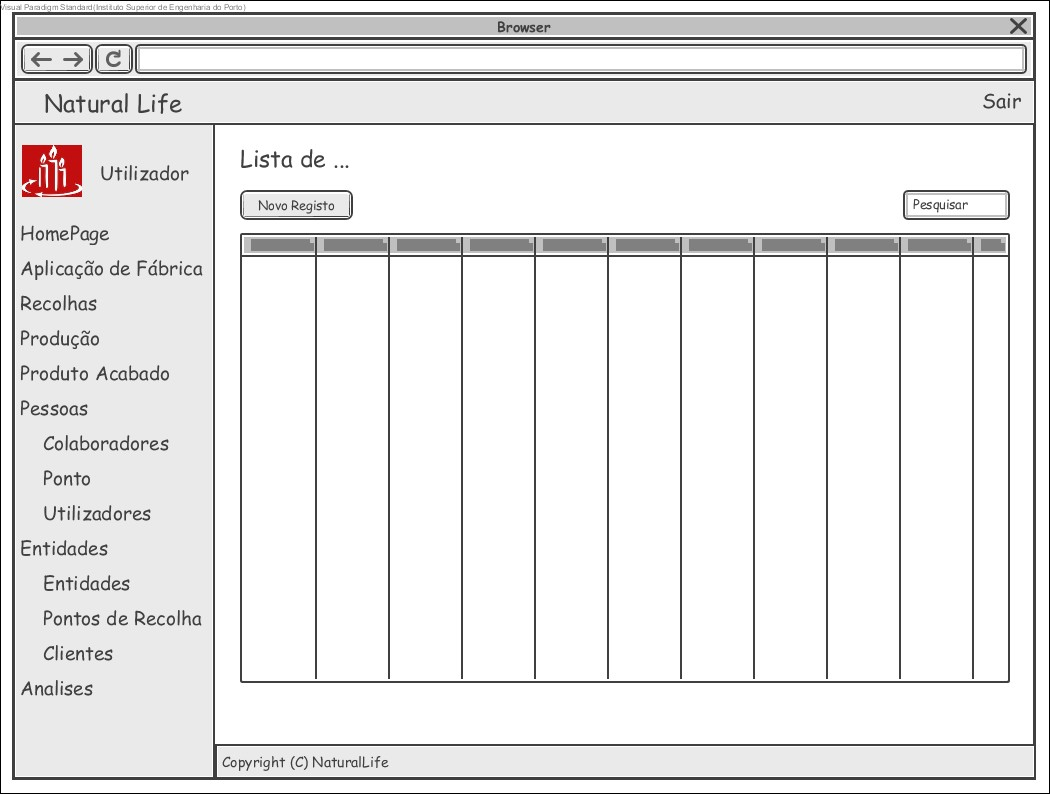
\includegraphics[width=0.60\textwidth,keepaspectratio]{figuras/Diagramas_vp/DI_Painel_1_Lista.jpg}
		\caption{Modelo da página de resultado de uma analise}
		\label{fig:di_analise} 
	\end{center}
\end{figure}

\subsubsection*{\textit{Models} compatíveis com o caso de uso}
Este caso de uso é apenas compatível com o \textit{model} Analises.

\subsubsection*{Fluxo do caso de utilização}
O caso de uso inicia-se quando o utilizador pressionar o botão executar da linha do registo que pretende executar. A página vai recarregar, fazendo aparacer o resultado da analise pedida, tal como demonstrado na figura \ref{fig:sd_executar analise}.


\begin{figure}[H] 
	\begin{center}
		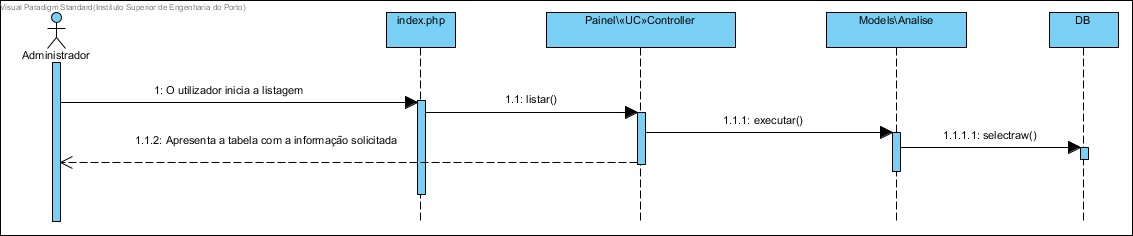
\includegraphics[width=\textwidth,keepaspectratio]{figuras/Diagramas_vp/SD_Painel_7_Executar_Analise.jpg}
		\caption{Diagrama de sequência para executar uma recolha}
		\label{fig:sd_executar analise} 
	\end{center}
\end{figure}